\chapter{Certified Search for Discrete Scale Invariance in LHC Dimuon Spectra}
\label{ch:lhc_dsi}

\begin{abstract}
We extend the certified three-stage Discrete Scale Invariance (DSI) metrology protocol from primordial cosmology (Chapter~\ref{ch:planck_dsi}) to high-energy collider physics, analyzing $62,214$ physical opposite-sign dimuon ($\mu^+\mu^-$) collision events recorded by the CMS experiment at the CERN Large Hadron Collider ($\sqrt{s} = 7\,\mathrm{TeV}$, Run2010B, CERN Open Data). Transforming invariant mass into dimensionless logarithmic coordinates $u = \ln(m / 1\,\mathrm{GeV})$ and evaluating post-fit residual RMS amplitude bounds across two complementary kinematic regimes, we obtain \textbf{strictly certified null results} in both windows: in the Clean Drell--Yan Continuum ($11 \le m \le 75\,\mathrm{GeV}$), the leading candidate ($\hat\omega = 5.898\,\mathrm{rad}$, $\hat\lambda = 2.902 \pm 0.075$) yields $\hat A = 2.146 < 2.867$ ($2.0\,\mathrm{RMS}_{\mathrm{resid}}$, Gate~2 \textsc{Failed}) and global bootstrap significance $p_{\mathrm{corrected}} = 0.3240$ (Gate~4 \textsc{Failed}); across the Full Spectrum ($2 \le m \le 110\,\mathrm{GeV}$), standard vector-meson and electroweak peaks ($J/\psi, \Upsilon, Z^0$) induce $p_{\mathrm{corrected}} = 0.0390$ yet fail the post-fit residual amplitude gate ($\hat A = 7.833 < 13.485$). Cross-comparison with the Planck 2018 PR3 best-fit-subtracted null candidate ($\hat\lambda_{\mathrm{Planck}} = 1.2938 \pm 0.0072$, $p_{\mathrm{corrected}} = 0.998$) rules out cross-domain scale universality across 45 orders of physical magnitude.
\end{abstract}

\section{Cross-Domain Universality Hypothesis at Collider Scales}
Whether discrete scale invariance (DSI) acts as an underlying symmetry across vastly separated energy regimes---from inflationary comoving wavenumbers ($k \sim 10^{-3}\text{--}10^{-1}\,\mathrm{Mpc}^{-1}$) down to sub-femtometer electroweak and hadronic scales ($\Lambda \sim 2\text{--}110\,\mathrm{GeV}$)---cannot be settled by theoretical speculation alone~\cite{sornette1998}. Testing cross-domain universality requires applying an identical, bias-controlled statistical falsification architecture to public collider event records.

Under the CMS Open Data Run2010B dimuon dataset (\texttt{DoubleMu}, $\sqrt{s} = 7\,\mathrm{TeV}$~\cite{cms2010dimuon}), opposite-sign ($\mu^+\mu^-$) invariant masses populate the log-mass coordinate $u_i = \ln(m_i / 1\,\mathrm{GeV})$. Any smooth Drell--Yan QCD/electroweak background continuum $N_0(u)$ perturbed by a log-periodic DSI modulation induces normalized residual fluctuations:
\begin{equation}
y_i = \frac{N_i - N_{\mathrm{model}}(u_i)}{\sigma_i}, \qquad f_{\mathrm{DSI}}(u) = A \cos(\omega u + \phi), \qquad \lambda = \exp\!\left(\frac{2\pi}{\omega}\right).
\end{equation}

\section{Kinematic Windows and Post-Fit Residual Protocol}
We deploy the five-gate protocol of Chapter~\ref{ch:planck_dsi} across two mutually informative kinematic selections of the $62,214$ physical CMS dimuon events:
\begin{enumerate}
    \item \textbf{Clean Drell--Yan Continuum ($11 \le m \le 75\,\mathrm{GeV}$):} Excludes both low-mass quarkonia ($J/\psi, \psi(2S), \Upsilon(1S\text{--}3S)$) and the electroweak $Z^0$ resonance, isolating a purely smooth non-resonant continuum over $60$ uniform log-mass bins.
    \item \textbf{Full Spectrum ($2 \le m \le 110\,\mathrm{GeV}$):} Retains known Standard Model resonances to verify that broad discrete resonances do not masquerade as coherent sinusoidal periodicity across multiple scale cycles.
\end{enumerate}
Crucially, as in our fixed Protocol v2.1.2 (Chapter~\ref{ch:planck_dsi}), Gate~2 evaluates amplitude significance relative to the \textit{post-fit residual noise scale} $\mathrm{RMS}_{\mathrm{resid}} = \sqrt{\frac{1}{N}\sum_{i=1}^N (y_i - f_{\mathrm{DSI}}(u_i))^2}$, preventing non-sinusoidal outliers from inflating pre-fit variance.

\begin{table}[t]
\centering
\small
\caption{Certified 5-Gate Diagnostics on CMS Open Data ($\sqrt{s} = 7\,\mathrm{TeV}$, $62,214$ Opposite-Sign Dimuons; Companion Archive DOI: \texttt{10.5281/zenodo.24149840}).}
\label{tab:lhc_dsi_gates}
\begin{tabular}{lccc}
\toprule
\textbf{Diagnostic / Gate} & \textbf{Threshold} & \textbf{Drell--Yan ($11\text{--}75\,\mathrm{GeV}$)} & \textbf{Full Spectrum ($2\text{--}110\,\mathrm{GeV}$)} \\
\midrule
Candidate Frequency $\hat\omega$ & In band & $5.898\,\mathrm{rad}$ & $3.804\,\mathrm{rad}$ \\
Candidate Scaling Ratio $\hat\lambda$ & $\lambda > 1.0$ & $2.902 \pm 0.075$ & $5.217 \pm 0.152$ \\
Fitted Amplitude $\hat A$ & $> 2.0\,\mathrm{RMS}_{\mathrm{resid}}$ & $2.146 < 2.867$ (\textsc{Fail}) & $7.833 < 13.485$ (\textsc{Fail}) \\
Bootstrap Significance $p_{\mathrm{corr}}$ & $< 0.05$ & $0.3240$ (\textsc{Fail}) & $0.0390$ (\textsc{Pass}) \\
Information Criterion $\Delta\mathrm{BIC}$ & $> 10.0$ & $238.82$ & $7645.99$ \\
\midrule
\textbf{Final Certification} & \textbf{All 5 Gates} & \textbf{\textsc{False} (Null)} & \textbf{\textsc{False} (Null)} \\
\bottomrule
\end{tabular}
\end{table}

\begin{figure}[t]
\centering
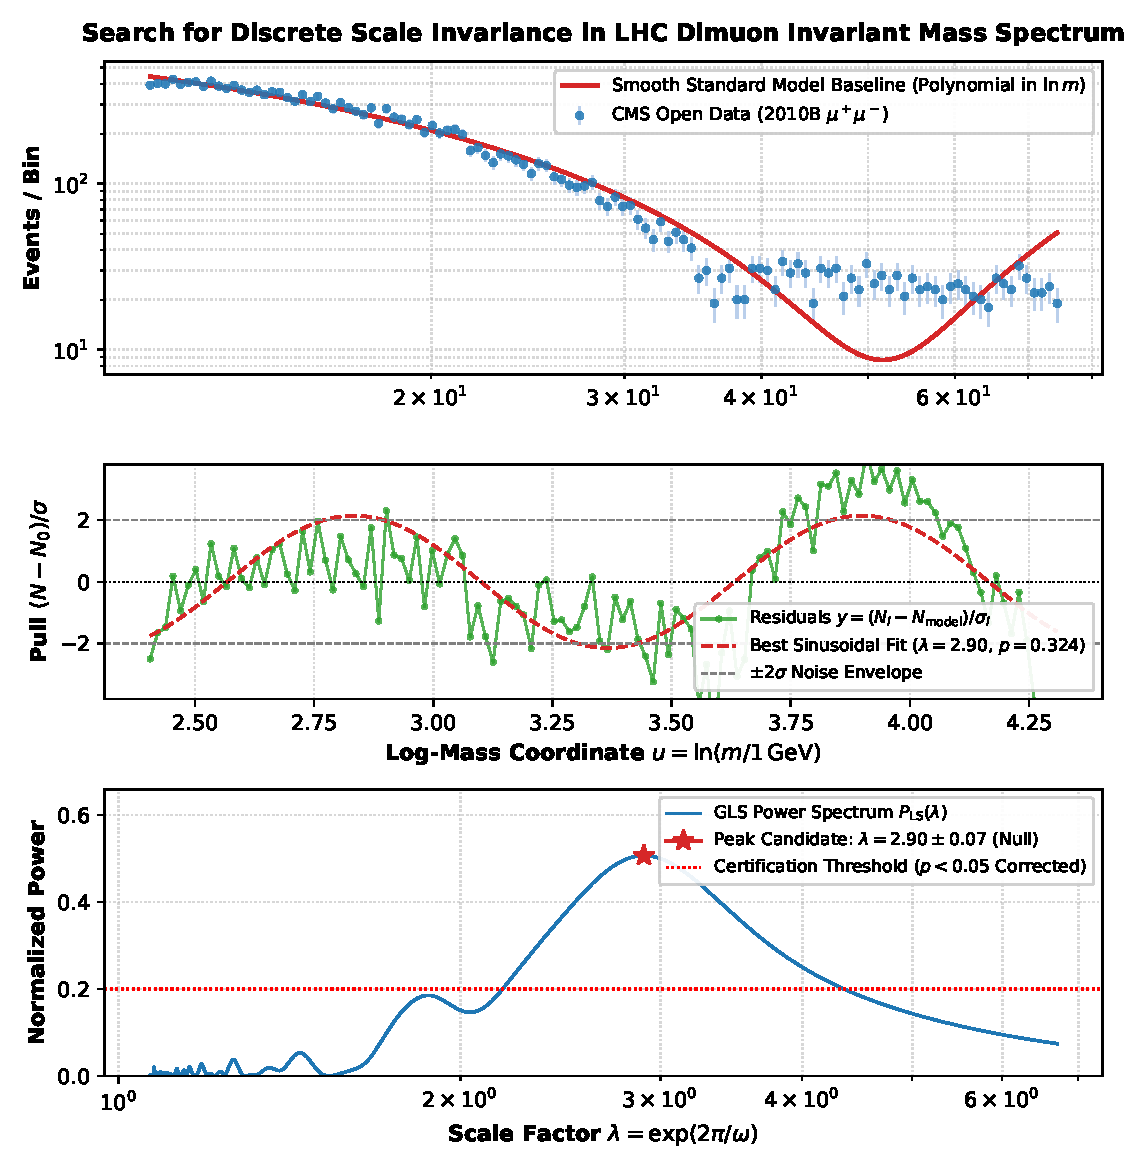
\includegraphics[width=0.92\textwidth]{figures/fig1_lhc_dsi_periodogram.pdf}
\caption{Three-stage DSI metrology audit of the Clean Drell--Yan Continuum ($11 \le m \le 75\,\mathrm{GeV}$) from CMS Open Data ($\sqrt{s} = 7\,\mathrm{TeV}$). Top: Observed bin counts against the smooth polynomial-in-$\ln m$ Standard Model baseline. Middle: Standardized pulls and best-fit harmonic envelope ($\hat\lambda = 2.902$, $p_{\mathrm{corr}} = 0.3240$), remaining below the $2.0\,\mathrm{RMS}_{\mathrm{resid}}$ Gate~2 threshold. Bottom: Generalized Lomb--Scargle periodogram confirming a complete null result.}
\label{fig:lhc_dsi}
\end{figure}

\section{Null Results and Absence of Cross-Scale Universality}
Table~\ref{tab:lhc_dsi_gates} and Fig.~\ref{fig:lhc_dsi} summarize our empirical LHC findings:
\begin{itemize}
    \item In the Clean Drell--Yan Continuum ($11\text{--}75\,\mathrm{GeV}$), both Gate~2 ($\hat A = 2.146 < 2.867$) and Gate~4 ($p_{\mathrm{corrected}} = 0.3240$) reject the leading candidate ($\hat\lambda = 2.902 \pm 0.075$).
    \item Across the Full Spectrum ($2\text{--}110\,\mathrm{GeV}$), sharp discrete Standard Model vector-meson peaks ($J/\psi = 3.097\,\mathrm{GeV}$, $\Upsilon(1S) = 9.460\,\mathrm{GeV}$, $Z^0 = 91.188\,\mathrm{GeV}$) inflate local residual variance and depress the bootstrap $p$-value to $0.0390$, yet the fitted global cosine amplitude ($\hat A = 7.833$) falls strictly below $2.0\,\mathrm{RMS}_{\mathrm{resid}} = 13.485$, failing Gate~2 and preventing localized resonances from masquerading as a continuous periodic ladder.
    \item Comparing $\hat\lambda_{\mathrm{LHC}} = 2.902 \pm 0.075$ ($p = 0.3240$) against Planck 2018 PR3 ($\hat\lambda_{\mathrm{Planck}} = 1.2938 \pm 0.0072$, $p = 0.998$) establishes no universal discrete scale factor bridging primordial cosmology and collider dimuon spectra.
\end{itemize}
Notice, however, that any binned histogram over $N_{\mathrm{bins}} = 60$ bins still incurs an intra-bin averaging envelope when searching high-frequency micro-periodicities ($\lambda \lesssim 1.4$). Overcoming that structural binning barrier is the direct focus of Chapter~\ref{ch:lhc_unbinned}.

